\documentclass[class=report, crop=false, 12pt,a4paper]{standalone}
\usepackage{graphicx}
\usepackage{float}
\usepackage{amsmath}
\usepackage{amssymb}
\usepackage{siunitx}
\usepackage{commath}
\usepackage[a4paper,width=150mm,top=25mm,bottom=25mm]{geometry}
\begin{document}
\section{Reynold's number}
Reynolds conducted experiments, in which he measured pressure drop and critical velocity in a variety of pipe diameters and with different fluids, and verified the importance of the parameter $\frac{\rho d \vec{U}}{\mu}$ later to be given his name. He found that, instead of a different critical velocity for each fluid and pipe, the onset of turbulence (i.e. transition) was determined by the achievement of the same critical value of Reynolds number, usually quoted as:
\begin{equation}
  Re_{d,crit} = 2300
\end{equation}
We note the confirmation of the empirical results regarding critical velocity because if:
\begin{equation}
  Re_{d,crit} = \frac{\rho d \vec{U}_{crit}}{\mu} = 2300
\end{equation}
then $\vec{U} \propto \frac{1}{d}$ for given $\rho$ and $\mu$ and $\vec{U}_{crit} \propto \mu$ for given $d$ and $\mu$.
\begin{figure}[H]
  \centering
  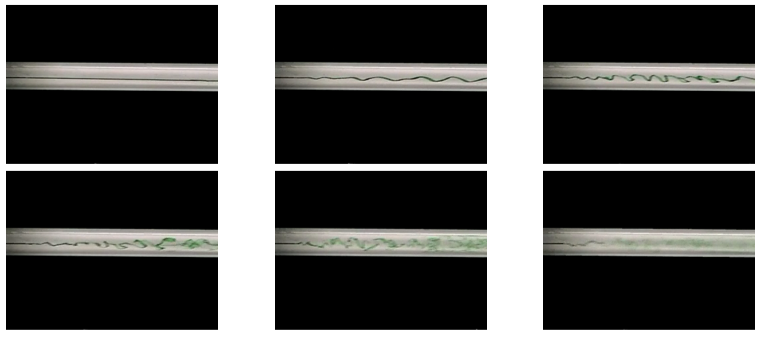
\includegraphics[width = 0.9 \textwidth]{../img/diagram78.png}
  \caption{}
\end{figure}
\begin{itemize}
  \item In this experiment water flows through a clear pipe with increasing speed
  \item Dye is injected through a small diameter tube at the left portion of the screen
  \item At low speed $ \left( Re < 2300 \right)$ the flow is laminar and the dye is a straight line
  \item As the speed increases, the dye stream becomes wavy (oscillatory laminar flow)
  \item At still higher speeds $\left(Re > 4000\right)$ the flow becomes turbulent and the dye stream is dispersed randomly throughout the flow
\end{itemize}
\section{Flow in pipes}
\subsection{Entrance region}
\begin{figure}[H]
  \centering
  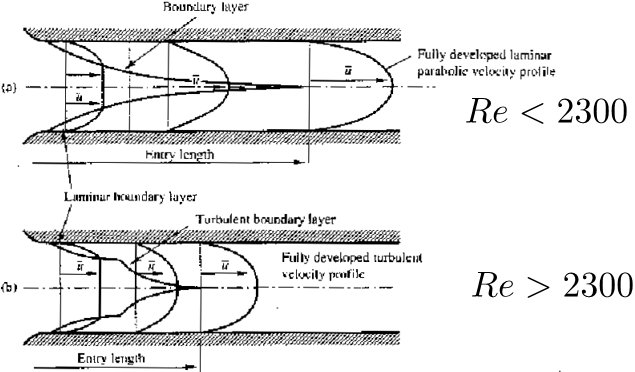
\includegraphics[width = 0.9 \textwidth]{../img/diagram79.png}
  \caption{}
\end{figure}
Reynolds number: $Re = \frac{\rho \vec{U} D}{\mu}$ where $D$ is the diameter.
\begin{figure}[H]
  \centering
  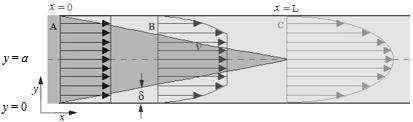
\includegraphics[width = 0.6 \textwidth]{../img/diagram80.png}
  \caption{}
\end{figure}
\begin{itemize}
  \item The nature of the flow in the entrance region and hence its length, depend on whether the fully-developed flow is laminar or turbulent
  \begin{itemize}
    \item \makebox[4cm]{$Re_d < 2300$:\hfill} Fully-developed flow should be laminar
    \item \makebox[4cm]{$Re_d > 2300$:\hfill} Fully-developed flow should be turbulent
    \item \makebox[4cm]{$2000 < Re_d < 3000$:\hfill} Transitional flow...
  \end{itemize}
  \item Figures given for laminar entry length variety
  \begin{itemize}
    \item \makebox[3cm]{\textit{Laghaar} quotes:\hfill} Entry length $=0.057 d Re_d$
    \item \makebox[3cm]{Rule of thumb:\hfill} Entry length $=100d$ minimum
  \end{itemize}
  \item For turbulent flow the fully-developed state is achieved much sooner (entry length less dependent on $Re_d$)
  \begin{itemize}
    \item \makebox[3cm]{Rule of thumb:\hfill} Entry length $=50d$ minimum
  \end{itemize}
\end{itemize}
\subsection{Shear stress}
What is the shear stress distribution in fully-developed pipe flows? Consider an axial cylindrical element of length $L$ within a pipe.
\begin{figure}[H]
  \centering
  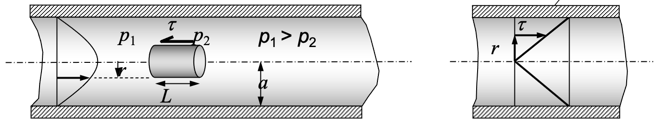
\includegraphics[width = 0.9 \textwidth]{../img/diagram81.png}
  \caption{}
\end{figure}
The forces due to pressure and shear (from velocity gradient) must balance out:
\begin{equation}
  p_1 \pi r^2 - p_2 \pi r^2 - \tau 2 \pi r L = 0 \rightarrow \tau = \frac{p_1 - p_2}{L} \frac{r}{2} = \frac{\Delta p}{L} \frac{r}{2} 
\end{equation}
This relationship is valid for both laminar and turbulent motion and shows that shear stress must vary linearly with radius $r$ in the pipe. The value of $\tau$ at the wall $\left( r = a \right)$ is: $\tau_w = \frac{\Delta p}{L} \frac{a}{2}$ so that: $\frac{\tau}{\tau_w} = \frac{r}{a}$. Wall shear stress can be measured by the pressure gradient in the pipe.
\subsection{Velocity profile}
Laminar motion $\left(Re < 2300\right)$. What is the velocity profile? If the motion is laminar, the shear stress is easily related to the velocity gradient through the dynamic viscosity, $\mu$.
\begin{figure}[H]
  \centering
  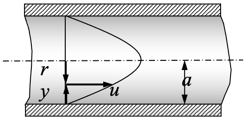
\includegraphics[width = 0.3 \textwidth]{../img/diagram82.png}
  \caption{}
\end{figure}
\begin{equation}
  \tau = \mu \frac{\dif u}{\dif y} \textrm{ where } y = a-r \textrm{ such that: } \dif y = -\dif r
\end{equation}
\begin{itemize}
  \item From previous result: $\tau = - \mu \frac{\dif u}{\dif r} = \frac{\Delta p}{L} \frac{r}{2}$
  \item Thus: $\dif u = - \frac{\Delta p}{2L} \frac{r}{\mu} \dif r$ which we can integrate to get: $u = - \frac{\Delta p}{4L\mu} r^2 + C$
  \item No slip boundary condition says: $u = 0$ at $ r = a \rightarrow C = \frac{\Delta p}{4 L \mu} a^2$
  \item Thus, finally: $u = \frac{1}{4\mu} \frac{\Delta p}{L} \left(a^2 - r^2\right)$ Parabolic velocity profile (\textit{Hagen-Poiseuille Law})
\end{itemize}
Segment V6.6 Laminar flow (Related to textbook section 6.9.3 - Steady, Laminar flow in circular tubes) The velocity distribution is parabolic for steady, laminar flow in circular tubes. A filament of dye is placed across a circular tube containing a very viscous liquid which is initially at rest. With the opening of a valve at the bottom of the tube the liquid starts to flow, and the parabolic velocity distribution is revealed. Although the flow is actually unsteady, it is quasi-steady since it is only slowly changing. Thus, at any instant in time the velocity distribution corresponds to the characteristic steady-flow parabolic distribution.
\subsection{Flow rate}
\begin{figure}[H]
  \centering
  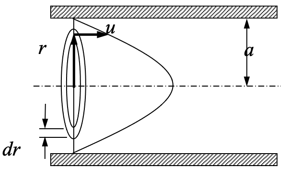
\includegraphics[width = 0.3 \textwidth]{../img/diagram83.png}
  \caption{}
\end{figure}
Parabolic velocity profile:
\begin{equation}
  u = \frac{1}{4\mu} \frac{\Delta p}{L} \left( a^2 - r^2\right)
\end{equation}
The maximum velocity $U_{max}$ occurs on the centre-line of the pipe (i.e. at $r=0$):
\begin{gather}
  U_{max} = \frac{1}{4\mu} \frac{\Delta p}{L}a^2\\
  \frac{u}{U_{max}} = \frac{a^2 - r^2}{a^2} \rightarrow \frac{u}{U_{max}} = 1 - \frac{r^2}{a^2}
\end{gather}
The mean velocity/flow rate is given by:
\begin{align}
  \vec{U} &= \frac{Q}{A} = \frac{\int_{0}^{a} \left(2\pi r u \right) \,\textrm{d}r}{\pi a^2}\\
  \vec{U} &= \frac{2\pi}{\pi a^2} \int_{0}^{a} \left(r u \right) \,\textrm{d}r = \frac{2}{a^2} \int_{0}^{a} \left(U_{\max} \left(1 - \frac{r^2}{a^2}\right)r\right) \,\textrm{d}r \\
  \vec{U} &= \frac{2U_{max}}{a^2} \int_{0}^{a} \left(r-\frac{r^3}{a^2}\right) \,\textrm{d}r\\
  \vec{U} &= \frac{2U_{max}}{a^2} \left[ \frac{r^2}{2} - \frac{r^4}{4a^2} \right]_0^a = \frac{2U_{max}}{a^2} \left[ \frac{a^2}{2} - \frac{a^4}{4a^2} \right] = \frac{U_{max}}{2} 
\end{align}
For a parabolic profile the mean velocity is hald the maximum velocity:
\begin{equation}
  u = \frac{1}{4\mu} \frac{\Delta p}{L} \left(a^2 - r^2\right) \makebox[1cm]{} U_{max} = \frac{1}{4\mu} \frac{\Delta p }{L} a^2 \makebox[1cm]{} \vec{U} = \frac{1}{8\mu}\frac{\Delta p}{L} a^2
\end{equation}
The volumetric flow rate is: 
\begin{equation}
  Q = \pi a^2 \vec{U} = \frac{\pi}{8\mu}\frac{\Delta p}{L} a^4
\end{equation}
This can be used as a basis for measuring $\mu$ if all the other parameters can be measured sufficiently accurately.
\section{Flow in pipes}
\subsection{Friction factor}
We have seen that the pressure loss in a pipe (whether laminar or turbulent) is related to the wall shear stress by:
\begin{equation}
  \tau_w = \frac{\Delta p}{L}\frac{a}{2}
\end{equation}
A dimensionless representation of the wall shear stress (and therefore the pressure gradient) is given by the defining a friction factor as the ratio of wall shear stress to dynamic pressure in the flow (based on mean velocity).
\begin{equation}
  f = \frac{\tau_w}{\frac{1}{2}\rho \vec{U}^2}
\end{equation}
\subsection{Pressure drop due to friction}
Generalised expression for pressure drop due to friction. We have seen from equilibrium considerations (for laminar or turbulent flow) that: 
\begin{equation}
  \tau_w = \frac{\Delta p}{L} \frac{a}{2} = \frac{\delta p}{L} \frac{d}{4}
\end{equation}
Thus,
\begin{equation}
  \Delta p = \frac{4L\tau_w}{d}\rightarrow \Delta p =\frac{4L}{d} f \frac{1}{2} \rho \vec{U}^2
\end{equation}
Hence:
\begin{equation}
  h_f = \frac{\Delta p}{\rho g} \rightarrow h_f = \frac{4L}{d} f \frac{\vec{U}^2}{2g} \label{darcys}
\end{equation}
Eq.\ref{darcys} is known as \textit{Darcy's} Formula. To work out the pressure drop due to friction in pipe flows, we need to know accurately the friction factor $f$.
\section{Friction factor for laminar flow in pipes}
Friction factor as a function of Reynolds number. Definition of friction factor (laminar or turbulent flow):
\begin{equation}
  f = \frac{\tau_w}{\frac{1}{2}\rho \vec{U}^2}
\end{equation}
For laminar flow we have:
\begin{equation}
  u = U_{max} \left(1-\frac{r^2}{a^2}\right) \makebox[1cm]{} \vec{U} = \frac{U_{max}}{2}
\end{equation}
Also:
\begin{gather}
  \tau_w = - \mu \left[\frac{\dif u}{\dif r}\right]_{r=a} = -\mu \left[\frac{-2\mu U_{max}a}{a^2}\right]_{r=a} = \frac{2\mu U_{max} a}{a^2} = \frac{2\mu U_{max}}{a} = \frac{4\mu U_{max}}{d}\\
  \tau_w = \frac{8\mu\vec{U}}{d}
\end{gather}
Thus, finally:
\begin{equation}
  f= \frac{\frac{8\mu\vec{U}}{d}}{\frac{1}{2}\rho \vec{U}^2} \rightarrow f = \frac{16\mu}{\rho d \vec{U}} \rightarrow f = \frac{16}{Re_d}
\end{equation}
\section{Laminar vs Turbulent profiles}
Segment V8.3 Laminar/Turbulent Velocity profiles (Related to textbook section 8.3.3 - Turbulent velocity profiles) The velocity profile for laminar flow in a pipe is quite different than that for turbulent flow. An approximation to the velocity profile in a a pipe is obtained by observing the motion of a dye streak placed across the pipe. With a viscous oil at Reynolds number of about 1, viscous effects dominate and it is easy to inject a relatively straight dye streak. The resulting laminar flow profile is parabolic. With water at Reynolds number of about 10000, inertial effects dominate and it is difficult to inject a straight dye streak. It is clear, however, that the turbulent velocity profile is not parabolic, but is more nearly uniform than for laminar flow. 
\end{document}